\documentclass[natbib]{sigplanconf}
\usepackage{xspace,pads,amsmath,math-cmds,
            math-envs,inference-rules,times,
            verbatim,alltt,multicol,proof,url}
\usepackage{epsfig}
\usepackage{code} 

\begin{document}

\conferenceinfo{POPL'08,}{January 7-12,2008, San Francisco, California, USA.} 
\copyrightyear{2008} 
\copyrightdata{978-1-59593-689-9/08/0001} 

\title{From Dirt to Shovels}
\subtitle{Fully Automatic Tool Generation from Ad Hoc Data}

\authorinfo{Kathleen Fisher}{
	   AT\&T Labs Research}
       {\mono{kfisher@research.att.com}}
\authorinfo{David Walker \qquad Kenny Q. Zhu}{
	   Princeton University}
       {\mono{{dpw,kzhu}@CS.Princeton.EDU}}
\authorinfo{Peter White}{
	   Galois, Inc.}
       {\mono{peter@galois.com}}
\newcommand{\cut}[1]{}
\newcommand{\reminder}[1]{{\it #1 }}
\newcommand{\poplversion}[1]{#1}
\newcommand{\trversion}[1]{}

\newcommand{\appref}[1]{Appendix~\ref{#1}}
\newcommand{\secref}[1]{Section~\ref{#1}}
\newcommand{\tblref}[1]{Table~\ref{#1}}
\newcommand{\figref}[1]{Figure~\ref{#1}}
\newcommand{\listingref}[1]{Listing~\ref{#1}}
%\newcommand{\pref}[1]{{page~\pageref{#1}}}

\newcommand{\eg}{{\em e.g.}}
\newcommand{\cf}{{\em cf.}}
\newcommand{\ie}{{\em i.e.}}
\newcommand{\etc}{{\em etc.\/}}
\newcommand{\naive}{na\"{\i}ve}
\newcommand{\role}{r\^{o}le}
\newcommand{\forte}{{fort\'{e}\/}}
\newcommand{\appr}{\~{}}

%\newcommand{\bftt}[1]{{\ttfamily\bfseries{}#1}}
\newcommand{\kw}[1]{\bftt{#1}}
\newcommand{\pads}{\textsc{pads}}
\newcommand{\padsc}{\textsc{pads/c}}
\newcommand{\ipads}{\textsc{ipads}}
\newcommand{\padsl}{\textsc{padsl}}
\newcommand{\blt}{\textsc{blt}}
\newcommand{\ddc}{\textsc{ddc}$^{\alpha}$}
\newcommand{\ddcold}{\textsc{ddc}}
\newcommand{\padsml}{\textsc{pads/ml}}
\newcommand{\padsmlbig}{\textsc{PADS/ML}}
\newcommand{\ddl}{\textsc{ddl}}
\newcommand{\C}{\textsc{c}}
\newcommand{\perl}{\textsc{perl}}
\newcommand{\ml}{\textsc{ml}}
\newcommand{\smlnj}{\textsc{sml/nj}}
\newcommand{\ocaml}{\textsc{o'caml}}
\newcommand{\java}{\textsc{java}}
\newcommand{\xml}{\textsc{xml}}
\newcommand{\xquery}{\textsc{xquery}}
\newcommand{\datascript}{\textsc{datascript}}
\newcommand{\packettypes}{\textsc{packettypes}}
\newcommand{\erlang}{\textsc{Erlang}}

\newcommand{\dibbler}{Sirius}
\newcommand{\ningaui}{Altair}
\newcommand{\darkstar}{Regulus}

%% \newcommand{\IParray}[4]{{\tt Parray} \; #1 \; \[#2, #3, #4\]}

\newcommand{\figHeight}[4]{\begin{figure}[tb]
	\centerline{
	            \epsfig{file=#1,height=#4}}
	\caption{#2}
	\label{#3}
	\end{figure}}


\maketitle{}

\begin{abstract}  
An {\em ad hoc data source} is any semistructured data source for
which useful data analysis and transformation tools are not 
readily available.  Such data must be queried, transformed and displayed by
systems administrators, computational biologists, financial analysts
and hosts of others on a regular basis.  
In this paper, we demonstrate that it is possible to generate a suite
of useful data processing tools, including a semi-structured query
engine, several format converters, a statistical analyzer and data
visualization routines directly from the ad hoc data itself, 
without any human intervention.  
The key technical contribution of the work is a multi-phase algorithm
that automatically infers the structure of an ad hoc data source and
produces a format specification in the \pads{} data description
language.  
Programmers wishing to implement custom data analysis tools
can use such descriptions to generate printing and parsing libraries
for the data.  Alternatively,  our software infrastructure will
push these descriptions through the \pads{} compiler, creating
format-dependent modules that, when linked with format-independent
algorithms for analysis and transformation, result in
fully functional tools.  We evaluate the performance of
our inference algorithm, showing it scales linearly
in the size of the training data --- completing in seconds, as opposed
to the hours or days it takes to write a description by hand.
We also evaluate the correctness of the algorithm, demonstrating that 
generating accurate descriptions often requires less than 5\% of the
available data.
\end{abstract}

\category{D.3.m}{Programming languages}{Miscellaneous}

\terms
Languages, Algorithms

\keywords
Data description languages, grammar induction, tool generation, ad hoc data


\section {Introduction}
\label{sec:intro}
\section{Introduction}
\label{sec:intro}

\datascript{}~\cite{gpce02}. \packettypes{}~\cite{sigcomm00}. \padsc{}~\cite{fisher+:pads}
and \padsml{}~\cite{mandelbaum+:padsml}. Bro\cite{paxson:bro}. These
are but a few of the many languages designed for describing data
formats. In his classic paper {\em The Next 700 Programming
  Languages}, 1966~\cite{landin:700}, Landin asserts that principled
programming language design involves thinking in terms of ``families
of languages'' and choosing from a ``well-mapped space.''  However,
when it comes to the domain of processing ad hoc data, there is no
well-mapped space and no systematic understanding of the family of
languages one might be dealing with.

In our previous work, we developed the data description calculus
\ddcold{} to capture the core features of many existing data
description languages~\cite{fisher+:next700ddl}, like \padsc{},
\packettypes{} and \datascript{}. Given the broad applicability of
\ddcold{}, we wanted to use it to define the semantics of
\padsml{}. However, the polymorphic types that we wished to include in
\padsml{} can not be formalized with \ddcold{}.  In addition, both
\padsc{} and \padsml{} generate tools from data format descriptions to
{\em print} data in the specified format. For
many applications, printing data correctly can be as important as
parsing it correctly. Yet, our previous work
specified only the type and parsing semantics of \ddcold{}. 

In this work, we address both of these limitations of
\ddcold{}. First, we extend \ddcold{} with abstractions over types to
create \ddc. In the process, we also improve the \ddc\ theory, as
noted in \secref{sec:ddc-sem}. The new \ddc provides basis for
specifying the semantics of \padsml{}. Second, we specify the a
printing semantics for the new \ddc{}.  We used this new
semantics to guide the \padsml{} implementation of printing.
\secref{sec:ddc} presents the extended \ddc{} calculus, focusing on
the semantics of polymorphic types for parsing and the key elements of
the printing semantics.  We show that both parsers and printers in the
\ddc{} are type correct and furthermore that parsers produce pairs of
parsed data and parse descriptors in {\em canonical form}, and that
printers, given data in canonical form, print successfully.

In summary, this work makes the following key contributions:
\begin{itemize}
\item We have defined the formal semantics of both \padsml{} parsers 
and printers. 
\item We have proven our generated code is type safe and
well-behaved as defined by a canonical forms theorem.
\end{itemize}

%%% Local Variables: 
%%% mode: latex
%%% TeX-master: "paper"
%%% End: 


\section{The Internal Format Description Language}
\label{sec:review}
\section{Review of PADS and LearnPADS}\label{sec:review}


\section{The Inference Algorithm}
\label{sec:inference}
% \subsection {Algorithm Overview}

\begin{figure}
\begin{center}
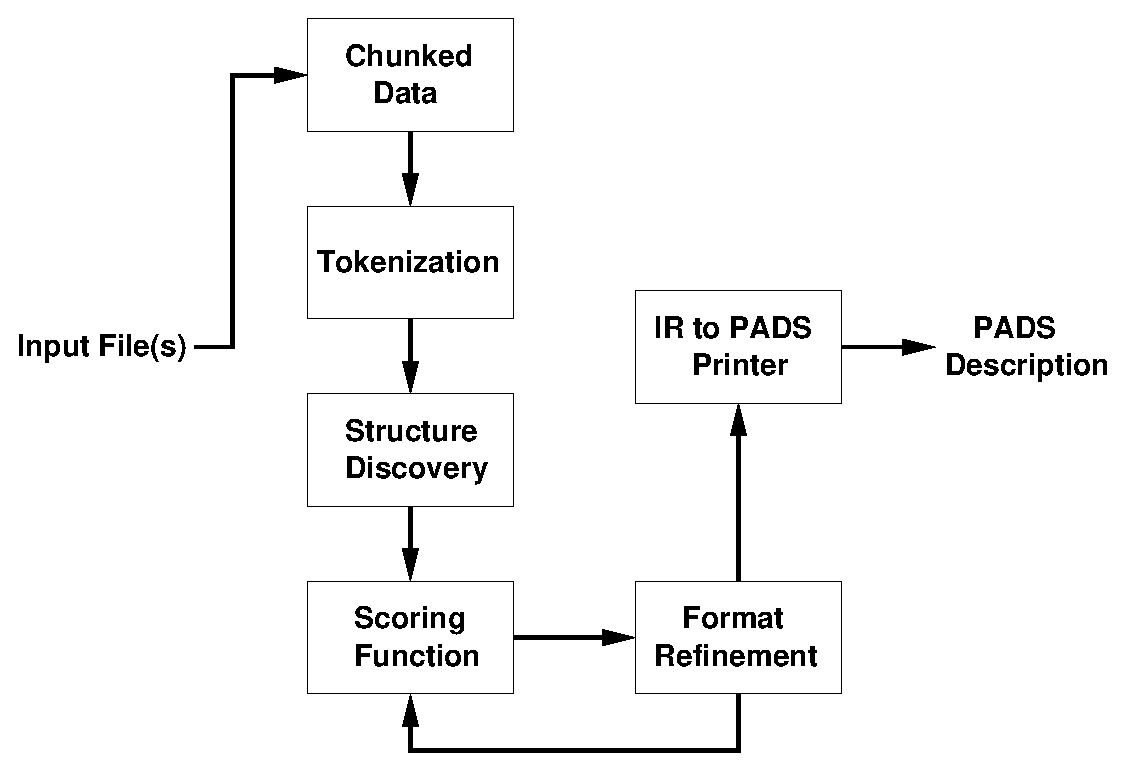
\epsfig{file=archi.eps, width=.9\columnwidth}
\caption{Architecture of the format inference engine}
\vspace*{-5mm}
\label{fig-archi}
\end{center}
\end{figure}

Figure \ref{fig-archi} gives an overview of our format inference
architecture. The input data, or ``training set,'' is first
``chunked'' into records where each record is a piece of recurrent
data such as a line, a paragraph, or a file (if the input consists of
multiple files).  The user specifies the unit of repetition when
invoking our learning tool.  Each record is then broken down into a
series of tokens where each token can be a punctuation symbol, a
number, a date, a time, or a number of other basic types.  Our
learning system has a basic tokenization scheme skewed toward systems
data, but users may specify a different scheme for their own domain
through a configuration file.  For example, computational biologists
may want to specify new base types for DNA strings or other common
recurring patterns.

In the structure discovery phase, we use a top-down, divide-and-conquer
scheme inspired in part by the work of Arasu on
information extraction from web pages~\cite{arasu+:sigmod03}. 
When a type constructor has been chosen, the data is partitioned accordingly
and the algorithm recursively analyzes subparts.  This
rough structure is represented in an intermediate representation (IR)
that has similar expressive power to the \pads{} language. 
The format refinement phase analyzes the IR produced by structure discovery
and repeatedly applies rewrite rules.  
In effect, this refinement phase is equivalent to a greedy, local search
procedure aimed at improving the quality of the inferred format.

\subsection {Chunking and Tokenization}

\begin{figure}
\begin{center}
\begin{tabular}{|l|l|}
\hline
Name   &  Description               \\ \hline\hline
Pint  &   Integer \\ 
Palpha & Alpha-numeric string including '$\_$' and '$-$' \\
Pip & IP address \\
Pemail & Email address \\
Pmac & Mac address \\
Pdate & Simple date format \\
Ptime & Simple time format \\
Ppath & File system path \\
Phostname & Hostname \\
Purl  & URL \\
PbXML & Beginning XML tag \\
PeXML & Ending XML tag \\
Pother & Punctuation character \\\hline
\end{tabular}

\caption{Basic token types in default configuration.}
\label{figure:base-types}
\end{center}
\end{figure}
 



    *  mention system parameterization for multiple tokenizations for different domains
    * mention current skew towards systems data
    * ignore problems in this section -- save that for discussion/future work section
    * mention stream of tokens generated for running example 

\subsection {Structure Discovery}

    *  role = quickly find a description in the "approximate area" of the correct description
    * explain structure of a generic "top-down" inference algorithm -- perhaps give pseudocode
    * explain our heuristics: generation of histograms, choice of struct, array, union, base type
    * grouping construct (introduce additional example as needed)
    * show (part of?) description of running example 

\subsection {Information-Theoretic Scoring}

    *  role = evaluate the "goodness" of the description relative to data
    * explain the information-theoretic principles
    * give the formulas 

\subsection {Structure Refinement}

    *  role = starting with the candidate structure, search for nearby descriptions that optimize an information theoretic scoring function
    * explain the 3 parts: value independent, value dependent, value independent
    * give (partial) list of rules used -- we need to work on notation for explaining these rules
    * illustrate several transformations using the running example
    * compare example after rewriting to the example from subsection 3.4 above
    * optional subsubsection: theory suggesting our algorithm is "correct" (we'd need a semantics for our IR then) 

\subsection {Finishing Up}

    * printing pads syntax and invoking toolchain

\section{Experimental Evaluation}
\label{sec:exp}
%\subsection{Objectives}
%
%The purpose of the experiment is to show the following points:
%\begin{itemize}
%\item the learning engine produces *accurate* and *concise* descriptions compared to a human
%expert's descriptions but costs just a fraction of the time; 
%\item it handles a variety of data formats; 
%\item the refinement step significantly improves the structure; 
%\item it is able to produce a description that is sufficiently accurate with 
%much smaller training sets (overfitting vs. underfitting); 
%\item demonstrate that there exists a correlation between sample size, execution time and accuracy,
%and the min sample size required to achieve certain accuracy correlates with the 
%data complexity.
%\end{itemize}

We conducted a series of experiments to study the learning algorithm
and measure its performance. In this section, we will show that
\begin{itemize}
\item the learning engine is capable of handing a variety of data formats;
\item while the initial structure discovery generates a reasonably
good candidate, the refinemnt phase siginificantly improves the
quality of the description through rewritings; 
\item the final output of the learning system is highly competitive
when compared with descriptions written by a human expert 
in terms of accuracy and conciseness; 
\item it is possible to learn from a small training set and produce
a relatively accurate description at a fraction of the cost;
\item there exists a positive correlation between the structural complexity
of the data and the minimum training size required to achieve certain
accuracy.
\end{itemize}

\subsection{Preliminaries}
\begin{table*}
\begin{center}
\begin{tabular}{|l|c|c|c|c|c|c|c|l|} \hline
Data source	& Chunks & Bytes	& Mode  &Header	& Array	& Group & Msgs 	& Comments \\ \hline \hline
1967Transactions.short	& 999	& 70929	& line	& no	& no	& no	& no	& transaction records \\ \hline
MER\_T01\_01.cvs	& 491	& 21731 & line  & yes	& no	& yes	& no	& comma-separated records\\ \hline
ai.3000		& 3000		& 293460 & line	& no	& no	& yes	& no	& web log of Amnesty International \\ \hline
asl.log &	1500	& 279600	& line	& no	& no	& yes	& no	& log file of Mac ASL \\ \hline	
boot.log	& 262	& 16241		& line	& no	& no	& no	& yes	& Mac OS boot log \\ \hline
crashreporter.log & 441	& 50152 	& line	& no	& no	& no	& yes	& original crashreporter daemon log \\ \hline
crashreporter.mod & 441	& 49255		& line	& no	& no	& no	& yes	& modified crashreporter daemon log \\ \hline
dibbler.1000	& 999	& 142607 	& line	& yes	& yes	& no	& no	& AT\&T phone provision data \\ \hline
ls-l.txt	& 35	& 1979		& line	& yes	& no	& no	& no	& Stdout from Unix command ls -l \\ \hline
netstat-an	& 202	& 14355		& block	& yes	& no	& no	& no	& output from netstat -an \\ \hline
page\_log	& 354	& 28170		& line	& no	& no	& no	& no	& printer logs \\ \hline
quarterlypersonalincome & 62	& 10177	& line	& yes	& no	& yes	& no	& spread sheet \\ \hline
railroad.txt	& 67	& 6218		& line	& yes	& yes	& yes	& no	& US rail road info \\ \hline
scrollkeeper.log & 671	& 66288		& line	& no	& no	& no	& yes	& log from cataloging system \\ \hline
windowserver\_last.log & 680	& 52394	& line	& no	& no	& no	& yes	& log from LoginWindow server on Mac \\ \hline
yum.txt		& 328	& 18221		& line	& no	& no	& no	& no	& log from package installer Yum \\ \hline
\end{tabular}
\caption{Benchmark profile} \label{tab:benchmarks}
\end{center}
\end{table*}

The original data sources we used in the experiments are listed in Table \ref{tab:benchmarks}.
These range from personal spread sheet, to government records to system logs, and 
represent vastly different formats. Some benchmarks are large with a few thousand
chunks or records, while others are small with just a few dozen lines. As we will see later
that the size of the data source has some implications in the training performance.
Most of the data files are line based, which means a line represent a data record, with
the exception of netstat-an in which data come in blocks or multiple lines.
Many of the formats include headers or footers which may complicate the descriptions.
From a human point of view, dibbler.1000 and railroad.txt consist of some special
character separated arrays. The ``Group'' column in the table shows if a data source
contain groupings delimited by special characters such as [, ], or quotations.
The ``Msgs'' column indicates whether the data source contains complex English text.
We include two versions of crashreporter.log: an original file ``crashreporter.log''
and ``crashreporter.log.mod'' with some of the date information replaced by ``-''. 
The latter has been used as an example in Section \ref{sec:review}. 

The system that executed the experiments is an 
Apple PowerBook G4 with a 1.67 GHz Processor and 512 MB DDR RAM 
running on Mac OS X 10.4 Tiger. 

\begin{table}
\begin{center}
\begin{tabular}{|l|c|c|c|} \hline
		&  Time to prod.	& MDL score 	& Parsing accuracy 	\\ \hline
HW IR	& -			& X		& -			\\ \hline	
HW PADS	& X			& -		& X			\\ \hline	
INF IR 	& -			& X		& -			\\ \hline
INF PADS & X			& -		& X			\\ \hline 
\end{tabular}
\caption{Measurement for the representations} \label{tab:metrics}
\end{center}
\end{table}

For any of the given data sources, there exists four different representations in 
our experiments: hand-rewritten PADS by human expert (HW PADS), hand-rewritten IR directly
translated from the HW PADS (HW IR), inferred IR from the learning engine (INF IR), and
inferred PADS description which is automatically translated from the INF IR (INF PADS). 
Note that as IR has a simplified language and is not as powerful as the full-fledged
PADS, the HW PADS does not use those features not available in IR and hence it is
not fully optimized. 
Nonetheless, the HW PADS and HW IR are thought to be ``pretty good'' descriptions of
the data and are used as control in the comparisons below. 
In general, we measure the time to produce the descriptions, the MDL scores of
and the parsing accuracy of the descriptions. 
Table \ref{tab:metrics} shows what we measure for each of the four representations.

\subsection{Experiments}
\begin{table*}
\begin{center}
\begin{tabular}{|l||r|r|r|r||r|r|c|} \hline
Formats 	 & Inf time (s) 	& Ref time (s) 	& Total time (s) & HW time (h) & Inf score 	&Ref score	& HW score \\ \hline \hline
1967Transactions.short & 0.20&      2.32&      2.56 	& 4.0 & 0.295 	&0.218 		&0.268		 \\ \hline
MER\_T01\_01.csv & 0.11&      2.80&      2.92 	& 0.5 & 0.648 	&0.112		&0.138		 \\ \hline
ai.3000          & 1.97&      26.35&     28.64	& 1.0 & 0.503	&0.332		&0.338		 \\ \hline
asl.log          & 2.90&      52.07&     55.26	& 1.0 & 0.630	&0.267		&0.361		 \\ \hline
boot.log         & 0.11&      2.40&      2.53 	& 1.0 & 0.620	&0.481		&0.703		 \\ \hline
crashreport.log   & 0.12&      3.58&      3.73 	& 2.0 & 0.607	&0.328		&0.348		 \\ \hline
crashreport.log.mod & 0.15&      3.83&      4.00 	& 2.0 & 0.612	&0.329		&0.347		 \\ \hline
dibbler.1000     & 2.24&      5.69&      8.00 	& 1.5 & 0.602	&0.470		&0.438		 \\ \hline
ls-l.txt         & 0.01&      0.10&      0.11 	& 1.0 & 0.559	&0.333		&0.401		 \\ \hline
netstat-an       & 0.07&      0.74&      0.82 	& 1.0 & 0.413	&0.394		&0.319		 \\ \hline
page\_log        & 0.08&      0.55&      0.65 	& 0.5 & 0.540	&0.107		&0.353		  \\ \hline
quarterlypersonalincome & 0.07&      5.11&      5.18 	& 48  & 0.544	&0.367		&0.354		\\ \hline
railroad.txt     & 0.06&      2.69&      2.76 	& 2.0 & 0.715	&0.506		&0.522		 \\ \hline
scrollkeeper.log & 0.13&      3.24&      3.40 	& 1.0 & 0.625	&0.354		&0.352		 \\ \hline
windowserver\_last.log  & 0.37&      9.65&      10.07	& 1.5 &0.618		&0.241		&0.267		 \\ \hline
yum.txt          & 0.11&      1.91&      2.03 	& 5.0 &0.827		&0.305		&0.474		 \\ \hline
\end{tabular}
\caption{Main results (Inf: structure inference, Ref: Refinement, HW: Hand-written)}
\label{tab:results}
\end{center}
\end{table*}

We first hand-coded all 16 formats in PADS and IR and measure timings and the scores 
of supposedly good descriptions (see HW time column in Table \ref{tab:results}). 
Several formats takes a few hours and up to 2 days(!) to complete because these were the very first 
PADS descriptions ever written by this person. It is obvious that coding description
in PADS is a daunting task for a novice despite that he is a computer science PhD!
To score a given HW IR, we wrote a simple recursive-descent parser with backtracking
for our IR so that the original data can be populated into the IR structure for
correct scoring of the data complexity which is the second component of the MDL score.
After a few attempts and modifications, the HW PADS descritions parses all 
the original data files with 100\% accuracy.

Next we ran the learning system on all 16 data files in their entirety, 
measured timings for structure inference, refinement and the total time which includes
printing out the PADS descriptions and other overhead. 
For accurate timing measurements, run each data format 10 times, and take the average 
after removing the best and the worst times.
We also recorded the scores of both the initial structure and the final structure after refinement.
All these measurements are included in Table \ref{tab:results} as well.
The generated PADS descriptions parses all original data files with 100\% accuracy,
therefore the correctness of the learned formats is guaranteed.

We can see from Table \ref{tab:results} that the learning system
generates correct descriptions of any given data in matters of seconds as opposed to
the hours and days taken by human beings. The execution time is roughly proportional
to the size of input data. For example, the largest data sources, ai.3000 and asl.log,
take also the longest time. Refinement typically takes more time than initial
structure discovery, as the functional dependency analysis in this phase is a quadratic
in the number of nodes in the IR and is the bottleneck of the algorithm. 
Note that all these timings are achieved with a completely unoptimized prototype system
with lots of overhead in book-keeping and I/Os.

%Compare these with the golden numbers from (1) in a big table. Show that the difference in scores
%can be siginificant in some cases hence room for improvement (may go into the discussion section)
%but timing advantage is huge and refinment improves initial struct a lot. Maybe also compare a case or
%two where the score from silver is comparable to golden and the actually description produced is also
%close to golden (to demo that our scoring makes some sense).
%Have a discussion here about while the learning tool may produce a longer description than human does,
%it parses all data correctly so the user is getting all these for free which is a tremendous benefit.
%Discuss 1967 where the inference does better than human.

Select random training sets of 5\%, 10\%, 15\%, ..., 80\% of 
the original data (3 sets for each size) and run learning tool end to end on 
them and take the average of 3 sets. 
Set threshhold levels of 90\% and 95\% accuracies and record how much training data (in percentage and
absolute terms) is needed for each golden format to achieve these accurary levels. Then relate this
to the normalized type complexty of the inferred IR of the entire data sets.
Plot graph of (timing, accuracy) vs. training size 
for a few examples, and show that we are doing a good job with reasonable sample size. The diagram should
show increasing accuracy and execution time as sample size goes up. Point out anomaly
where the abolute training size is too small (e.g. for ls-l.txt which only has 35 lines) which results
in overfitting. ls-l.txt is also problematic as it has a header in the first line and if that is not included
in the training set, the data will not parse.

\begin{figure}
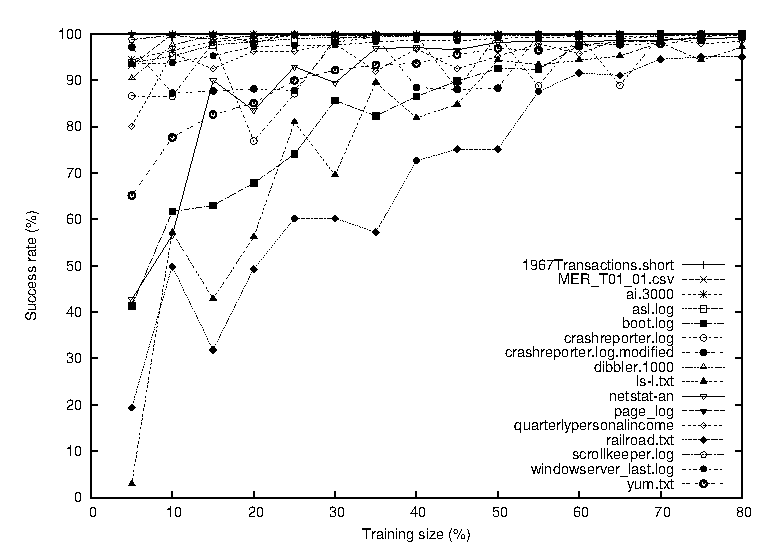
\epsfig{file=successrate.eps, width=\columnwidth}
\caption{Success rates of training sets}
\end{figure}

\begin{figure}
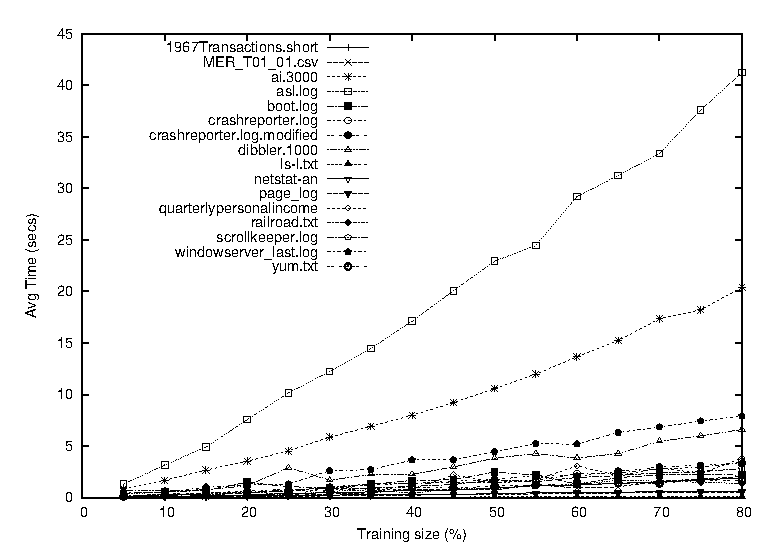
\epsfig{file=traintime.eps, width=\columnwidth}
\caption{Execution times of training sets}
\end{figure}

\begin{table}
\begin{center}
\begin{tabular}{|l|r|l|c|c|} \hline
Title 			& Bytes 	& Ty Comp	& 90\% 		& 95\% \\ \hline \hline
1967Transactions.short	& 70929		& 0.0003	& 5		& 5 			\\ \hline
MER\_T01\_01.csv        & 21731 	& 0.0037	& 5		& 5\\ \hline
ai.3000                 & 293460 	& 0.0004	& 5		& 10\\ \hline
asl.log                 & 279600	& 0.0012	& 5		& 10\\ \hline
boot.log                & 16241		& 0.0213	& 40		& 50\\ \hline
crashreporter.log       & 50152 	& 0.0052	& 5		& 5\\ \hline
crashreporter.log.mod   & 49255		& 0.0053	& 5		& 5\\ \hline
dibbler.1000            & 142607 	& 0.0001	& 5		& 5\\ \hline
ls-l.txt                & 1979		& 0.0461	& 50		& 70\\ \hline
netstat-an              & 14355		& 0.0118	& 20		& 25\\ \hline
page\_log               & 28170		& 0.0032	& 5		& 5\\ \hline
quarterlypersonalincome & 10177		& 0.017		& 10		& 20\\ \hline
railroad.txt            & 6218		& 0.0485	& 60		& 85\\ \hline
scrollkeeper.log        & 66288		& 0.002		& 5		& 5\\ \hline
windowserver\_last.log  & 52394		& 0.0084	& 5		& 10\\ \hline
yum.txt                 & 18221		& 0.0124	& 30		& 40\\ \hline
\end{tabular}
\caption{Min Training size (\%) vs. required accuracy}
\end{center}
\end{table}

\begin{figure}
\begin{center}
\epsfig{file=traintycomp.eps, width=\columnwidth}
\caption{Correlation between structure complexity of 
the data and minimum training size required}
\end{center}
\end{figure}


\section{Discussion}
\label{sec:discussion}
\subsection{Related Work}

\subsection {Current and Future Work}

thoughts on problems with tokenization; information theory; partial
descriptions; user interface; recursion; more experimentation with a
broader range of formats


\section{Related Work}
\label{sec:related}
Researchers have been studying {\em grammar induction}, the process of
inferring descriptions of text-based data, for decades.  Nevertheless,
the work we present in this paper represents an important and novel 
contribution to the field for three key reasons:

\begin{enumerate}
\item Our system solves {\em a new end-to-end problem} not treated in
past work --- the problem of generating an extensible suite of fully
functional data processing tools directly from ad hoc data.  
%%We can
%%currently generate an XML translator, a normalizing reformatter, a
%%graphing tool, a full query engine allowing users to write arbitrary XQueries
%%against the ad hoc data, an accumulator tool, and
%%programming libraries for parsing, printing and data validation.
Generating this suite requires the combination of three elements:
grammar induction, automatic intermediate representation generation
and type-directed programming.  A key contribution of this work is the
conception, development and evaluation of this end-to-end system.

%%After surveying
%%experts at the CAGI 2007 workshop on grammar induction, where we
%%presented a two-page overview of our system~\cite{burke+:cagi07}, and
%%searching the literature, we could find no existing system that
%%provides this end-to-end functionality.

\item Past work on grammar induction has focused primarily on
either (1) theoretical problems, (2) natural language processing, 
(3) web page analysis, or
(4) XML typing.  Our work tackles an understudied domain, that of complex system
logs and other ad hoc data sources.  Since ad hoc data has
different characteristics from the previously studied domains, naive
adaptations of the existing algorithms are unlikely to be %the most
effective.  
%%As the evaluation in this paper shows, our system is tuned
%%to perform well on ad hoc data, particularly system logs and
%%networking data.  
%%One of the conclusions of the chair of the CAGI 2007
%%workshop, presented in the final discussion session of the workshop,
%%was that ``ad hoc data'' was indeed a new domain for the study of
%%grammar induction and that more research in this area was an important
%%future direction for the community.

\item  From a technical standpoint, we developed a new top-down 
structure-discovery algorithm and showed how to combine that 
productively with a classic bottom-up rewriting system based on 
the minimum description length principle. We demonstrate that our
new algorithm has good practical properties on ad hoc data sources:  
it usually infers correct descriptions on a small amount of training
data and its performance scales linearly relative to the amount of training
data used.
\end{enumerate}

\noindent
%We presented a two-page overview of our system~\cite{burke+:cagi07} at
%the CAGI 2007 workshop on grammar induction. 
In the rest of this section, we analyze
the most closely related work in more depth.

\paragraph*{Traditional Grammar Induction.}
Classic grammar induction algorithms \cite{vidal:gisurvey} 
can be divided into two classes: those that require both
positive and negative examples to discover a grammar and those that
only require positive examples. The problem our system solves is the latter;
negative examples of ad hoc data sources are not available in
practice.  Consequently, effective theoretical algorithms for learning
from both positive and negative
examples such as RPNI~\cite{rpni}
%~\cite{lemay+:tree-transducers,rpni,raeymaekers+:learning-tree-languages},
are not applicable in our context.

Unfortunately, an early result by \citet{gold:inference} showed
that perfect grammar induction is impossible for any superfinite class
of languages when the algorithm has no access to negative examples.  A
{\em superfinite} class of languages is any set of languages that
includes all finite languages and at least one infinite
language. Hence, all the most familiar classes of languages, including
regular expressions, context free grammars and PADS are superfinite.
There are two main tactics one can use to avoid this negative
result: 
(1) use domain knowledge to explicitly limit the class of languages to a
non-superfinite class, or
(2) give up on perfect language identification and instead settle for {\em approximate
identification}~\cite{wharton:approximate-language-identification}
through the use of probabilistic language models.

Examples of non-trivial, non-superfinite
language classes with known inference algorithms include
k-reversible languages~\cite{angluin:revesible-language-inference},
%k-testable regular languages~\cite{garcia+:k-testable-languages},
SOREs and CHAREs~\cite{bex+:dtd-inference}.
None of these languages and the associated algorithms 
are a good fit for inferring PADS descriptions (even the
regular subset of PADS without dependencies and constraints).  
For example, ad hoc data is unlikely to be reversible and hence
k-reversible languages are not relevant.  
%K-testable regular languages are
%more relevant, but algorithms for inferring them
%operate by finding a finite automaton and converting that 
%automaton into a regular expression.  Unfortunately, the conversion process
%often leads to overly verbose regular expressions, sometimes 
%exponential in the size of the automaton~\cite{bex+:dtd-inference}. 
SOREs are a subset of the k-testable
regular languages with a linear-size translation from automata to
regular expressions, but they carry the restriction that each symbol
in the regular expression appear at most once.  A cursory glance at
our hand-written PADS descriptions reveals that many such descriptions
include repeated use of the same symbol.  Finally, it appears that
CHAREs restrict the nesting of regular expression operators too severely to 
be of much use to us.  For example, when $a$, $b$, and $c$ are atomic symbols,
even the simple expression $(ab + c)*$ is not a CHARE.

Given the difficulty of finding useful non-superfinite language classes,
it is reasonable to turn to algorithms for approximate
inference that use probabilistic models.    
Classic examples of such procedures include work by~\citet{stolcke94inducing} 
%%{\em insert other references here -- see Hong thesis related work
%%for other work...} 
and 
\citet{hong:thesis}.  These and a number of other algorithms
operate by repeatedly rewriting a candidate grammar (or set of candidate
grammars) until an objective function is optimized.
If the training data for the learning system is the strings
$s_1$, $s_2$, $\ldots$, $s_n$, these algorithms normally start their
process using the grammar $s_1 + s_2 + \cdots + s_n$.  Consequently,  
an enormous number of different rewrites may apply to the
initial candidate grammar.  Our structure refinement
phase avoids these problems 
because it is preceded by a highly efficient
histogram-based structure-discovery algorithm 
that identifies a good candidate grammar from which to start the search.  
%%Another interesting, non-standard element of our algorithm is the way 
%%it is tuned to include specialized rules for finding constraints and 
%%rewrite tokens.
%%These rules are very useful in the domain of ad hoc data; different
%%considerations are appropriate in other domains such as XML or HTML.

%% is also tuned in a variety of ways to make it effective

%% The effectiveness of structure-discovery allows us to 
%% simplify our search algorithm and cut down the search space we 
%% look at substantially.  In addition to worrying about
%% performance considerations, we tuned our structure refinement phase
%% specifically for ad hoc data by including domain-specific rules
%% for finding constraints and 
%% dependencies as well as those for introducing constants, enumerations and
%% good basic types/tokens that cannot be found effectively at earlier stages.
%% Some of these rules are needed in our system, but not other systems
%% that work in different domains, because
%% tokenization is highly ambiguous in ad hoc data.
%% Our initial tokenization and structure-discovery algorithms often 
%% over-generalize and this over-generalization must be undone during
%% the rewriting phase.  {\em NOTE: end of that paragraph was highly  run-on}

Another category of algorithms are those that learn various kinds of
automata as opposed to regular expressions or 
grammars~\cite{denis:learning-regular-languages,rpni,raeymaekers+:learning-tree-languages}.  
One difficulty with adapting these algorithms to our task is that 
we would need to convert the inferred automata into a 
grammatical representation so that we can
present the result to users and funnel it
to our tool-generation infrastructure.
Unfortunately, in theory, conversion from automata into
regular expressions can result in an exponential blowup in the
size of the representation.
Moreover, a substantial blowup appears to be relatively common in
practice~\cite{bex+:dtd-inference}.  Consequently, these algorithms
are not appropriate for our domain.



%% developed another system for information extraction from web pages
%% based on learning ($k$,$l$)-Contextual Tree Languages.  They show that
%% these tree languages can be learned from positive examples 
%% (from which one may infer they are not superfinite) and apply
%% their techniques to the problem of information extraction.  One of the
%% difficulties they face involves estimating the parameters involved in

  
%% {\em NOTE: I'm leaving out reference to denis:learning-regular-languages (see
%% pads.bib file).
%% Vincent Danos mentioned it but it contains no references to any real data.
%% It's interesting theoretical result that infers a new kind of automaton.
%% This automaton will likely have the same potential difficulties 
%% (possibly exponential explosion -- I haven't prove that though) 
%% when conversion to regular expressions happens. Anyway, I just didn't
%% want to bother studying the paper because they're so much other stuff
%% that is more relevant.  basically, I just couldn't figure out how to cram
%% the reference in elegantly.  I actually couldn't even figure out when I skimmed
%% the paper whether or not it uses both positive and negative examples.
%% It gets compared to RPNI, so I think it must use negative examples.
%% }

%% One disadvantage of such
%% techniques is that the initial state is large (representing
%% the entire training data set explicitly) and the search space is 
%% enormous.  Nevertheless, bottom-up state-merging is often used because
%% it has been difficult to find an effective state-splitting algorithm.
%% Our histogram-based structure-discovery procedure is a new state-splitting
%% algorithm that appears to work well on ad hoc data when coupled with
%% bottom-up rewriting.


%% The classic grammar induction problem~\cite{vidal:gisurvey} requires we find an
%% algorithm that discovers a grammar $G$ given a set of
%% positive examples $R+$ (example strings in the language to be inferred)
%% and a set of negative examples $R-$ (example strings {\em not}
%% in the language to be inferred).  To be more specific, in the limit,
%% as the sets of positive and negative examples grow, the
%% algorithm is expected to converge on the language that defines them.  
%% Unfortunately, very early on,
%% Gold~\cite{gold:inference} proved a key negative result about this problem:  If
%% the algorithm is presented with no negative examples, grammar
%% induction for any super-finite class of languages is impossible.
%% A {\em super-finite} class of languages is any set of languages
%% that includes all finite languages and at least one infinite language.
%% All the most familiar classes of languages, including regular expressions, 
%% context free grammars and PADS, fall into this class.

%% Traditional
%% Some traditional grammar induction algorithms assume that
%% both positive and negative training data
%% One way to categorize research in traditional
%% grammar induction is to ask whether the research in question
%% assumes that both positive and negative training data is available
%% or whether only positive training data is available.

%% analyze the assumptions made
%% about the training data.  
%% Very early in the study of grammar induction, Gold proved a key
%% negative result:


%% Other researchers have defined grammar induction algorithms that use
%% bottom-up rewriting to search through description space for an optimal
%% description.  Many of these techniques, such as 
%% require the availability of both
%% positive and negative examples.  In our context, negative examples
%% never exist, making such techniques inapplicable.
%% % since Gold's early result proved the
%% %impossibility of {\em perfect} grammar induction for any useful family of
%% %languages when no negative examples are
%% %available~\cite{gold:inference}.  
%% However, others, such as Stolcke and
%% Omohundro~\cite{stolcke94inducing} and Hong~\cite{hong01using}, do not
%% assume the existence of negative examples.  These and a number of other systems
%% search through solution space using
%% state-merging rewriting rules.  One disadvantage of such
%% techniques is that the initial state is large (representing
%% the entire training data set explicitly) and the search space is 
%% enormous.  Nevertheless, bottom-up state-merging is often used because
%% it has been difficult to find an effective state-splitting algorithm.
%% Our histogram-based structure-discovery procedure is a new state-splitting
%% algorithm that appears to work well on ad hoc data when coupled with
%% bottom-up rewriting.

% State-merging rewriting rules seem to be
% more popular than 
% that use bottom-up rewriting to find good grammars may suffer from the
% problem of running into local maxima.  The rewriting component of our
% algorithm can also run into a local maximum, but because we start with
% a relatively good candidate generated from our recursive, top-down
% algorithm, this does not appear to be much of a problem for us.  We
% also believe that combining top-down structure-discovery with
% bottom-up rewriting has the potential to deal with larger data sources
% than a pure bottom-up approach.  Our empirical experiments demonstrate
% that the top-down structure-discovery phase is extremely efficient
% when compared with the cost of rewriting.  However, proposals for
% bottom-up-only inference techniques use the (possibly enormous) data
% source itself as the first description.  We are unaware of other
% systems that combine two techniques similar to ours.


%% ; De La Higuera
%% surveys some recent trends~\cite{higuera01current}.  However,
%% our system is unique in two important ways.  First, our inference
%% algorithm does not stand alone; it is part of the more general \pads{}
%% programming environment.  The fusion of the
%% \pads{} system, including its automatic data representation generation,
%% its error detection facilities, its generic programming environment, 
%% and its powerful tool suite, together with grammar induction
%% is one of our key contributions.  Second, many researchers have
%% focused either on grammar induction for natural language processing or
%% for information extraction from \xml{} or \html{} documents.  In
%% contrast, we focus on ad hoc data sources such as system logs and
%% scientific data sets. Ad hoc data is substantially less
%% structured syntactically than \xml{}, and yet, unlike natural language, it is
%% possible to assign our data sources accurate, compact descriptions. After
%% searching the literature and consulting
%% with experts in grammar induction at the CAGI 2007
%% workshop, where we presented a two page overview of our system~\cite{burke+:cagi07},
%% we could find no existing work comparable to ours.

% Third, from a
% technical standpoint, we developed a new top-down structure-discovery
% algorithm and showed how to combine that productively with a
% classic bottom-up rewriting systems based on the minimum description
% length principle.  In what follows, we compare our system more
% specifically to the most closely related work of other researchers.

\paragraph*{Information Extraction.}

The basic goal of an information extraction system is to find and
separate the interesting and relevant bits of information (the
needles) from a haystack of data.  Such systems are fundamentally
different from ours, in that they choose which bits of information to
extract, while we learn a description of the entirety of a data
source, leaving the choice about which pieces are interesting to
down-stream applications.  Of course, this option is only feasible
because we target ad hoc data, which is fairly structured and dense in
useful information, rather than web pages or free text, which are the
usual targets for information extraction systems. 

A common approach to information extraction involves an inductive
learning process in which a user manually tags the relevant data in sample documents.
An example might be highlighting product names and prices on a
collection of shopping web pages from a particular site.  The learning
system then uses these labelled documents in two ways: first, to
decide which bits of information should be extracted from the page
(\ie, product names and prices), and second, to construct a
\textit{wrapper} function to extract those bits of information from
similar pages.  Soderland's WHISK system (\citeyear{soderland:whisk}) is an
example of such an extraction system.  It is particularly general as
it makes few assumptions about the form of the source text,
operating over structured data, stylized text such as Craig's List
descriptions, or free-form text.  WHISK differs from our system in
that it requires user labeling and then only extracts a collection of
tuples from the data source rather than returning the complete
structure of the data source.


Kushmerick and
colleagues (\citeyear{kushmerick-phd1997,KushmerickWD97:Wrapper}) focus on
more structured data to reduce the amount of labeling required during
training.  In particular, this work assumes the labelled pages conform
to one of six different templates, the most well-developed of which
has the form of a header, followed by a sequence of K-tuples each of
which is flanked by a pair of begin and end tags, followed by a
trailer.  For such documents, the system generates a wrapper to
extract the K-tuples.  
% To limit the amount of labeling, the system
% has provisions to automatically tag the desired tuples using {\it
% recognizers}, which are imperfect, but reusable heuristics for finding
% atomic pieces of data such as country names or phone numbers.  Such
% recognizers mean the user has to select which set of recognizers to
% use for a particular extraction task instead of labeling pages by
% hand.  The system requires one recognizer to be {\it perfect}, meaning
% it generates neither false positives nor false negatives.  It then
% uses a process called {\it corroboration} to correct the mistakes of
% the other recognisers.  The system is not robust in the presence of
% missing data, and it is not clear how it would handle multiple
% instances of the same kind of data within a single tuple. This
% approach differs from ours in that it requires the data to comform to
% one of a fixed collection of templates.  In addition, the 
% templates that support corroboration will only return relational data,
% whereas our system will return semi-structured data.
The use of fixed templates and the primary focus on relational data makes this
work quite different from ours.

\citet{muslea+:active-learning} tackle a similar
problem, but strive to reduce the amount of labeling by having the
learning system chose which documents to have the user label,
selecting documents by their probative value.  \citet{borkar+:text-segmentation} uses hand-labelled training
examples and a user-specified set of desired features to train Hidden
Markov Models to select the desired features from similar documents.
This work is quite successful at learning to select the relevant
features of addresses and bibliographic citations from a variety of
input formats. 
% Various researchers have leveraged the syntactic
% regularity and verbosity of XML/HTML to reduce the amount of user
% annotations required to train information extraction systems targetted
% at web pages~\cite{Ambite+:ariadne,doorenbos+:shopbot}.
% Work by Ireson {\em et al.}~\cite{ireson+:ml-evaluation} investigates
% how information extraction systems should be evaluated.  Soderland's
% WHISK paper~\cite{soderland:whisk} and Kushmerick's
% theis~\cite{kushmerick-phd1997} both contain detailed descriptions of
% other information extraction systems.  
In general, systems that depend
upon labeling are unlikely to be helpful in our context; rather than
spending time explicitly labeling documents, the user might as well
write a PADS description by hand.

% Another type of information extraction system strives to provide a
% high-level semantic characterization of the content of natural
% language documents to guide information retrieval
% queries~\cite{gubanov+:structural-text-search,rus+:information-capture}.
% This work differs from ours in that it is building a semantic rather
% than a syntatic description of the source data.

More closely related are various efforts to identify tabular data 
either from free-form text~\cite{Ng+:texttables,Pinto+:texttables} or
from web pages~\cite{Lerman+:webtables}.  These approaches typically
use hand-labelled examples to train machine learning systems to
identify the tables.  They then use heuristics specific to tabular
data to extract the tuples contained within those tables.  The portion
of this work related to identifying structured data from within more
free-form documents is complementary to ours.  The portion responsible
for deconstructing the identified tables uses more specific
domain-knowledge related to the form of tables than we do.

Web pages generated in response to queries tend to be formed by
sloting the resulting tuples into a standard template.  Another line
of work aims to separate such templates from the payload
data~\cite{arasu+:sigmod03,Cresenzi+:roadrunner}.  
Arasu and Garcia-Molina %~\cite{arasu+:sigmod03}
use a top-down grammar induction
algorithm somewhat similar to our rough structure-inference phase
(though it does not use histograms),
but has no description-rewriting engine.  
%However, in certain ways, Arasu has a much easier task than we do as html
%documents have far more regular structure than ad hoc data sources do.
This algorithm exploits the hierarchical nesting
structure of \xml{} documents in essential ways
and so cannot be applied directly to ad hoc data.  
%For example,
%we use histograms to summarize the contents of data chunks whereas
%Arasu does not.  In addition, a substantial portion of our system
%is a description rewriting engine, which Arasu seems not to need.  






% For further reading on
% information extraction from web pages, Hong's
% thesis~\cite{hong:thesis} includes an informative survey.  Though,
% Arasu's work and TSIMMIS appear more closely related to our work than
% the others Hong mentions.


\paragraph*{XML Type Inference.}
Many researchers have studied the problem of learning
a schema such as a DTD or XSchema from a collection 
of XML
documents~\cite{bex+:dtd-inference,bex+:inferring-xml-schema,fernau:learning-xml,garofalakis+:xtract}.  
At a high level, this task is similar to the format inference component of our system.  
However, the details differ because XML has different characteristics
from ad hoc data.  One difference is that XML documents come in a well-nested tree 
shape, with obvious delimiters defining the structure.  
A second important difference is that the appropriate tokenization for
a given ad hoc data source is often not known in advance.  
%%One of our strategies for dealing with
%%these ambiguities is to define simple approximate tokens for use
%%in the tokenization phase, but then to employ a collection of 
%%rules to improve token ({\em i.e.}, base type) choices in the rewriting phase
%%when more contextual information is available.  
In contrast,
tokens in XML documents are clearly demarcated using angle bracket syntax.
%%A third difference is that XML documents are often organized such that
%%the structure of a child node is dependent on its parent or grandparent.
%%In contrast, in the flatter ad hoc data we have considered, dependencies
%%generally arise between siblings -- some data item to the left influences
%%the structure of data to the right.  
As a result of these differences,
XML inference algorithms cannot be used ``off-the-shelf'' for understanding
the structure of ad hoc data.  They must be modified, tuned and
empirically evaluated on this new task.

One line of research on schema inference for XML makes use of the 
observation that 99\% of the content models for XML nodes are defined as
SOREs or CHAREs~\cite{martens+:expressiveness-xml-schema}. 
%(recall, these
%are heavily restricted forms of regular expressions).  
This observation allows \citet{bex+:dtd-inference} to define
an efficient algorithm for inferring concise DTDs.  Later 
\citet{bex+:inferring-xml-schema} build on this work 
by showing how to infer $k$-local XML Schema definitions also based on
SORES.  A $k$-local definition allows node content to depend on the parent
tag, grandparent tag, etc. (up to $k$ levels for some fixed $k$).
As mentioned earlier, hand-written PADS descriptions do not generally obey
the SOREs or CHAREs restriction, nor are they generally arranged with a nesting
structure that suggests $k$-local inference will be particularly useful.
The successful application of these techniques to XML data reinforces 
the idea that the ad hoc data we analyze has quite different characteristics
from XML, and therefore the ad hoc data inference problem merits study
independent of the XML inference problem.

XTRACT~\cite{garofalakis+:xtract} is another system for inferring DTDs
for XML documents.  It operates in three phases: generalization,
factoring and MDL optimization.  The first phase plays a role similar to
our structure discovery phase in that it generates a
collection of candidate structures from a series of XML examples.
This generalization phase searches for patterns in XML
data; it is tuned using the authors' knowledge of common DTD
structures.  Factoring decreases the size of generated candidate DTDs;
some of the factoring rules resemble our rewriting rules.
Finally, they tackle the MDL optimization problem by mapping the
problem into an instance of the NP-complete Facility Location Problem,
which they solve using a quadratic approximation algorithm.
Our MDL-guided rewriting problem considers a more general set of
rewriting rules and hence we cannot reuse their technique.

%% Another related problem of great interest in the XML and database world
%% involves finding a mapping between two data sources with different schema.
%% \citet{doan+:disparate-data-sources} is one example amongst
%% many which attempts to solve this problem using a machine learning approach.
%% While some of our PADS tools do involve translations between
%% different formats, our learning system does not attempt to discover
%% translation tools for which the output is guaranteed to match 
%% the characteristics of a second data set.


\paragraph*{Other work.}
Potter's Wheel~\cite{raman+:potterwheel} is a system that attempts to
help users find and purge errors from
relational data sources.  It does so through the use of a spread-sheet
style interface, but in the background, a grammar inference algorithm
infers the structure of the input data, which may be ``ad hoc,'' 
somewhat like ours.  This inference algorithm operates by
enumerating all possible sequences of base types that appear
in the training data.  
%As in our work,
%users can specify custom base types, and search for a description
%is based on the minimum description length principle.  
Since Potter's Wheel is aimed at processing
relational data, they only infer \cd{struct} types
as opposed to enumerations, arrays, switches or unions.  

The TSIMMIS project~\cite{chawathe+:tsimmis} aims to
allow users to manage and query collections of heterogeneous, ad hoc
data sources.  TSIMMIS sits on top of the Rufus
system~\cite{shoens+:rufus}, which supports automatic classification
of data sources based on features such as the presence of certain
keywords, magic numbers appearing at the beginning of files and file
type.  
%The sources are classified using categories such as ``email''
%and ``C program.''  
This sort of classification is materially
different from the syntactic analysis we have developed.



\section{Conclusions}
\label{sec:conclusion}
\section{Conclusion} 
\label{sec:conclusion}

Ad hoc data is pervasive and valuable: in industry, in medicine, and
in scientific research.  Such data tends to have poor documentation,
to contain various kinds of errors, and to be voluminous.  Unlike
well-behaved data in standardized relational or \xml{} formats, such
data has little or no tool support, forcing data analysts and
scientists to waste valuable time writing brittle custom code, even if
all they want to do is convert their data into a well-behaved format.
To improve the situation, various researchers have developed data
description languages such as \pads{}, \datascript{}, and
\packettypes{}.  Such languages allow analysts to write terse,
declarative descriptions of ad hoc data.  A compiler then generates a
parser and customized tools.  Because these languages are tailored to
their domain, they can provide useful services automatically while a
more general purpose tool, such as \lex{}/\yacc{} or \perl{}, cannot.

In the spirit of Landin, we have taken the first steps toward
specifying a semantics for this class of languages by defining the
data description calculus \ddc{}.  This calculus, which is a dependent
type theory with a simple set of orthogonal primitives, is expressive
enough to describe the features of \pads{}, \datascript{}, and
\packettypes{}.  In keeping with the spirit of the data description
languages, our semantics is transformational: instead of simply
recognizing a collection of input strings, we specify how to transform
those strings into canonical in-memory representations annotated with
error information.  Furthermore, we prove that the error information
is meaningful, allowing analysts to rely on the error summaries rather
than having to re-vet the data by-hand.

We have already used the semantics to identify bugs in the
implementation of \padsc{} and to highlight areas where \padsc{}
sacrifices safety for speed.  We have also used the semantics as a guide
for the design of a whole new language, \padsml{}, designed
specifically for functional programmers.  In the future, we hope 
\ddc{} will serve as a solid foundation for the next 700 data 
description languages to come.


\section*{Acknowledgments}

Our work benefited greatly from thoughts and comments from
Alex Aiken, David Blei, David Burke, Vikas Kedia, John Launchbury, Chris Ramming, 
Rob Schapire
and the organizers and attendees of the CAGI 2007 Workshop on Grammar
Induction.

This material is based upon work 
supported by DARPA under grant FA8750-07-C-0014
and the NSF
   under grants 0612147 and 0615062.
Any opinions, findings, and conclusions or recommendations
   expressed in this material are those of the authors and do not
   necessarily reflect the views of DARPA or the NSF.


\bibliographystyle{plainnat}
\begin{thebibliography}{37}
\providecommand{\natexlab}[1]{#1}
\providecommand{\url}[1]{\texttt{#1}}
\expandafter\ifx\csname urlstyle\endcsname\relax
  \providecommand{\doi}[1]{doi: #1}\else
  \providecommand{\doi}{doi: \begingroup \urlstyle{rm}\Url}\fi

\bibitem[Angluin(1982)]{angluin:revesible-language-inference}
Dana Angluin.
\newblock Inference of reversible languages.
\newblock \emph{Journal of the ACM}, 29\penalty0 (3):\penalty0 741--765, 1982.

\bibitem[Arasu and Garcia-Molina(2003)]{arasu+:sigmod03}
Arvind Arasu and Hector Garcia-Molina.
\newblock Extracting structured data from web pages.
\newblock In \emph{{SIGMOD}}, pages 337--348, 2003.

\bibitem[Bex et~al.(2006)Bex, Neven, Schwentick, and Tuyls]{bex+:dtd-inference}
Geert~Jan Bex, Frank Neven, Thomas Schwentick, and Karl Tuyls.
\newblock Inference of concise {DTDs} from {XML} data.
\newblock In \emph{{VLDB}}, pages 115--126, 2006.

\bibitem[Bex et~al.(2007)Bex, Neven, and
  Vansummeren]{bex+:inferring-xml-schema}
Geert~Jan Bex, Frank Neven, and Stijn Vansummeren.
\newblock Inferring {XML} schema definitions from {XML} data.
\newblock In \emph{{VLDB}}, pages 998--1009, 2007.

\bibitem[Borkar et~al.(2001)Borkar, Deshmukh, and
  Sarawagi]{borkar+:text-segmentation}
Vinayak Borkar, Kaustubh Deshmukh, and Sunita Sarawagi.
\newblock Automatic segmentation of text into structured records.
\newblock In \emph{{SIGMOD}}, pages 175--186, New York, NY, USA, 2001.

\bibitem[Burke et~al.(2007)Burke, Fisher, Walker, White, and
  Zhu]{burke+:cagi07}
David Burke, Kathleen Fisher, David Walker, Peter White, and Kenny~Q. Zhu.
\newblock Towards 1-click tool generation with {PADS}.
\newblock In \emph{{CAGI}}, Corvallis, OR, June 2007.

\bibitem[Chawathe et~al.(1994)Chawathe, Garcia-Molina, Hammer, Ireland,
  Papakonstantinou, Ullman, and Widom]{chawathe+:tsimmis}
Sudarshan Chawathe, Hector Garcia-Molina, Joachim Hammer, Kelly Ireland, Yannis
  Papakonstantinou, Jeffrey~D. Ullman, and Jennifer Widom.
\newblock The {TSIMMIS} project: Integration of heterogeneous information
  sources.
\newblock In \emph{16th Meeting of the Information Processing Society of
  Japan}, pages 7--18, Tokyo, Japan, 1994.

\bibitem[Crescenzi et~al.(2001)Crescenzi, Mecca, and
  Merialdo]{Cresenzi+:roadrunner}
Valter Crescenzi, Giansalvatore Mecca, and Paolo Merialdo.
\newblock Roadrunner: Towards automatic data extraction from large web sites.
\newblock In \emph{{VLDB}}, pages 109--118, San Francisco, CA, USA, 2001.

\bibitem[Denis et~al.(2004)Denis, Lemay, and
  Terlutte]{denis:learning-regular-languages}
Fran\c{c}ois Denis, Aur{\'e}lien Lemay, and Alain Terlutte.
\newblock Learning regular languages using {RFSAs}.
\newblock \emph{Theoretical Computer Science}, 313\penalty0 (2):\penalty0
  267--294, 2004.

\bibitem[Fern\'andez et~al.(2006)Fern\'andez, Fisher, Gruber, and
  Mandelbaum.]{fernandez+:padx}
Mary~F. Fern\'andez, Kathleen Fisher, Robert Gruber, and Yitzhak Mandelbaum.
\newblock {PADX}: Querying large-scale ad hoc data with {XQuery}.
\newblock In \emph{{PLAN-X}}, January 2006.

\bibitem[Fernau(2001)]{fernau:learning-xml}
Henning Fernau.
\newblock Learning {XML} grammars.
\newblock In \emph{{MLDM}}, pages 73--87, 2001.

\bibitem[Fisher and Gruber(2005)]{fisher+:pads}
Kathleen Fisher and Robert Gruber.
\newblock {PADS}: A domain specific language for processing ad hoc data.
\newblock In \emph{{PLDI}}, pages 295--304, June 2005.

\bibitem[Fisher et~al.(2006)Fisher, Mandelbaum, and Walker]{fisher+:popl06}
Kathleen Fisher, Yitzhak Mandelbaum, and David Walker.
\newblock The next 700 data description languages.
\newblock In \emph{{POPL}}, January 2006.

\bibitem[Garofalakis et~al.(2000)Garofalakis, Gionis, Rastogi, Seshadri, and
  Shim]{garofalakis+:xtract}
Minos~N. Garofalakis, Aristides Gionis, Rajeev Rastogi, S.~Seshadri, and
  Kyuseok Shim.
\newblock {XTRACT}: A system for extracting document type descriptors from
  {XML} documents.
\newblock In \emph{{SIGMOD}}, pages 165--176, 2000.

\bibitem[Gold(1967)]{gold:inference}
E.~M. Gold.
\newblock Language identification in the limit.
\newblock \emph{Information and Control}, 10\penalty0 (5):\penalty0 447--474,
  1967.

\bibitem[Gr\"{u}nwald(2007)]{mdlbook}
Peter~D. Gr\"{u}nwald.
\newblock \emph{The Minimum Description Length Principle}.
\newblock {MIT Press}, May 2007.

\bibitem[Hong(2002)]{hong:thesis}
Theodore~W. Hong.
\newblock \emph{Grammatical Inference for Information Extraction and
  Visualisation on the Web}.
\newblock Ph.D. Thesis, Imperial College London, 2002.

\bibitem[Huhtala et~al.(1999)Huhtala, K{\"a}rkk{\"a}inen, Porkka, and
  Toivonen]{TANE-HKPT99}
Yk{\"a} Huhtala, Juha K{\"a}rkk{\"a}inen, Pasi Porkka, and Hannu Toivonen.
\newblock {TANE}: An efficient algorithm for discovering functional and
  approximate dependencies.
\newblock \emph{The Computer Journal}, 42\penalty0 (2):\penalty0 100--111,
  1999.

\bibitem[Hutchens and Alder(1998)]{hutchens98finding}
Jason~L. Hutchens and Michael~D. Alder.
\newblock Finding structure via compression.
\newblock In David M.~W. Powers, editor, \emph{Proceedings of the Joint
  Conference on New Methods in Language Processing and Computational Natural
  Language Learning}, pages 79--82. 1998.

\bibitem[Kushmerick(1997)]{kushmerick-phd1997}
N.~Kushmerick.
\newblock \emph{Wrapper induction for information extraction}.
\newblock PhD thesis, University of Washington, 1997.
\newblock Department of Computer Science and Engineering.

\bibitem[Kushmerick et~al.(1997)Kushmerick, Weld, and
  Doorenbos]{KushmerickWD97:Wrapper}
Nicholas Kushmerick, Daniel~S. Weld, and Robert~B. Doorenbos.
\newblock Wrapper induction for information extraction.
\newblock In \emph{{IJCAI}}, pages 729--737, 1997.

\bibitem[Lerman et~al.(2004)Lerman, Getoor, Minton, and
  Knoblock]{Lerman+:webtables}
Kristina Lerman, Lise Getoor, Steven Minton, and Craig Knoblock.
\newblock Using the structure of web sites for automatic segmentation of
  tables.
\newblock In \emph{{SIGMOD}}, pages 119--130, New York, NY, USA, 2004.

\bibitem[Lin(1991)]{Lin91:divergence}
J.~Lin.
\newblock Divergence measures based on the {Shannon} entropy.
\newblock \emph{IEEE Transactions on Information Theory}, 37\penalty0
  (1):\penalty0 145--151, 1991.

\bibitem[Mandelbaum et~al.(2007)Mandelbaum, Fisher, Walker, Fernandez, and
  Gleyzer]{mandelbaum+:pads-ml}
Yitzhak Mandelbaum, Kathleen Fisher, David Walker, Mary Fernandez, and Artem
  Gleyzer.
\newblock {PADS/ML}: {A} functional data description language.
\newblock In \emph{{POPL}}, January 2007.

\bibitem[Martens et~al.(2006)Martens, Neven, Schwentick, and
  Bex]{martens+:expressiveness-xml-schema}
Wim Martens, Frank Neven, Thomas Schwentick, and Geert~Jan Bex.
\newblock Expressiveness and complexity of {XML} schema.
\newblock \emph{ACM Transactions on Database Systems}, 31\penalty0
  (3):\penalty0 770--813, 2006.

\bibitem[Muslea et~al.(2003)Muslea, Minton, and
  Knoblock]{muslea+:active-learning}
Ion Muslea, Steve Minton, and Craig Knoblock.
\newblock Active learning with strong and weak views: a case study on wrapper
  induction.
\newblock In \emph{{IJCAI}}, pages 415--420, 2003.

\bibitem[Ng et~al.(1999)Ng, Lim, and Koo]{Ng+:texttables}
Hwee~Tou Ng, Chung~Yong Lim, and Jessica Li~Teng Koo.
\newblock Learning to recognize tables in free text.
\newblock In \emph{{ACL}}, pages 443--450, Morristown, NJ, USA, 1999.

\bibitem[Oncina and Garcia(1992)]{rpni}
J.~Oncina and P.~Garcia.
\newblock Inferring regular languages in polynomial updated time.
\newblock \emph{Machine Perception and Artificial Intelligence}, 1:\penalty0
  29--61, 1992.

\bibitem[PADS Project()]{padsweb}
PADS Project.
\newblock {PADS} project.
\newblock {\url{http://www.padsproj.org/}}, 2007.

\bibitem[Pinto et~al.(2003)Pinto, McCallum, Wei, and Croft]{Pinto+:texttables}
David Pinto, Andrew McCallum, Xing Wei, and W.~Bruce Croft.
\newblock Table extraction using conditional random fields.
\newblock In \emph{SIGIR}, pages 235--242, New York, NY, USA, 2003.

\bibitem[Raeymaekers et~al.(2005)Raeymaekers, Bruynooghe, and den
  Bussche]{raeymaekers+:learning-tree-languages}
Stefan Raeymaekers, Maurice Bruynooghe, and Jan~Van den Bussche.
\newblock Learning (k, l)-contextual tree languages for information extraction.
\newblock In \emph{{ECML}}, pages 305--316, 2005.

\bibitem[Raman and Hellerstein(2001)]{raman+:potterwheel}
Vijayshankar Raman and Joseph~M. Hellerstein.
\newblock Potter's wheel: An interactive data cleaning system.
\newblock In \emph{{VLDB}}, pages 381 -- 390, 2001.

\bibitem[Shoens et~al.(1993)Shoens, Luniewski, Schwarz, Stamos, and
  Joachim~Thomas]{shoens+:rufus}
Kurt~A. Shoens, Allen Luniewski, Peter~M. Schwarz, James~W. Stamos, and
  II~Joachim~Thomas.
\newblock The {Rufus} system: Information organization for semi-structured
  data.
\newblock In \emph{{VLDB}}, pages 97--107, San Francisco, CA, USA, 1993.

\bibitem[Soderland(1999)]{soderland:whisk}
Stephen Soderland.
\newblock Learning information extraction rules for semi-structured and free
  text.
\newblock \emph{Machine Learning}, 34\penalty0 (1-3):\penalty0 233--272, 1999.

\bibitem[Stolcke and Omohundro(1994)]{stolcke94inducing}
Andreas Stolcke and Stephen Omohundro.
\newblock Inducing probabilistic grammars by bayesian model merging.
\newblock In \emph{{ICGI}}, pages 106--118, 1994.

\bibitem[Vidal(1994)]{vidal:gisurvey}
Enrique Vidal.
\newblock Grammatical inference: An introduction survey.
\newblock In \emph{{ICGI}}, pages 1--4, 1994.

\bibitem[Wharton(1974)]{wharton:approximate-language-identification}
R.~M. Wharton.
\newblock Approximate language identification.
\newblock \emph{Information and Control}, 26\penalty0 (3):\penalty0 236--255,
  1974.

\end{thebibliography}
\end{document}


